\documentclass{article}
\usepackage[utf8]{inputenc}
\usepackage{amsmath}
\usepackage{listings}
\usepackage{appendix}
\usepackage{geometry}
\usepackage{graphicx}
\usepackage{subfig}
\usepackage{gensymb}
\usepackage{cancel}
\usepackage{physics}
\usepackage[colorlinks=true]{hyperref}
\usepackage{xcolor}
\definecolor{codegreen}{rgb}{0,0.6,0}
\definecolor{codegray}{rgb}{0.5,0.5,0.5}
\definecolor{codepurple}{rgb}{0.58,0,0.82}
\definecolor{backcolour}{rgb}{0.95,0.95,0.92}
\lstdefinestyle{mystyle}{
    backgroundcolor=\color{backcolour},   
    commentstyle=\color{codegreen},
    keywordstyle=\color{magenta},
    numberstyle=\tiny\color{codegray},
    stringstyle=\color{codepurple},
    basicstyle=\ttfamily\footnotesize,
    breakatwhitespace=false,         
    breaklines=true,                 
    captionpos=b,                    
    keepspaces=true,                 
    numbers=left,                    
    numbersep=5pt,                  
    showspaces=false,                
    showstringspaces=false,
    showtabs=false,                  
    tabsize=2
}

\lstset{style=mystyle}
\title{%
Project 3 - Machine Learnt Spam Filter\\
\Large Using different supervised Machine Learning Methods \\
\Large to create a simple Spam Filter for e-mails \\
\large FYS-STK3155 at University of Oslo}
\author{Simen Løken}
\date{December 2020}
\footskip = 90pt
\topmargin = -40pt

\begin{document}
\nocite{Nb}
\nocite{lecture}
\nocite{svm}

\maketitle
{
  \hypersetup{linkcolor=black}
  \tableofcontents
}
\newpage
\section{Abstract}
In this report, we'll start by introducing different machine learning models, their properties and their algorithms. From there, we will discuss our problem at length and what we wish to achieve, before pitting all methods up against each other as a text-classifier for spam-filtering. After having trained our models, we check their accuracy scores and find that the Random Forest Classifier performs the best with a 0.95 accuracy rating. We'll then run custom strings against our created model, to get a feel for which model can best handle spam, and we find that the Random Forest Classifier is the best overall.
\section{Introduction}
Since the dawn of mail, mankind has had to contend with junk mail filling their postboxes. Try as you might, put up a sticker, threaten the postman, stand guard outside your postbox, the junk mail always finds a way. Luckily however, we are in the digital era now. There is no longer any reason to despise your postman, you can now instead despise strangers online filling your digital postbox with unsolicited spam mail. \newline 
I'm sure this problem needs no motivation. We've all had to deal with spam mail, and although the spam filters of providers like Google have gotten very good, that wasn't always the case. Whether it be cryptocurrency left in an account somewhere expiring, a prince from a far-away land feeling generous or a suspicious million dollar give away from John Smith in exchange for account information, we've all experienced it. \newline
In this report, we'll therefore try to build a spam-classifier from the ground up, using tried and true machine learning methods for our purposes. We'll discuss these methods at length, some new, and some we've already discussed, before diving in to the models themselves. We'll be training them on the UCI Spambase \cite{data} data set, which contains 57 different features/attributes and a label denoting whether or not it is spam. The data set is a typical "bag-of-words" data set, meaning it only uses a select few words and their frequency in a given email. It additionally also contains measurements of special characters and upper-case usage. \newline
Once our models are up and running, we'll check their accuracy scores in order to gauge how successful they are, before pitting them up against never-before-seen spam written by yours truly, to see if they hold up. After gathering all required data, we'll do one final look-over of all methods and their results, and try to find which method is best for our purposes.
\newpage
\section{Theory}
Given that we're going to be looking at and weighing a set of different methods and how they relate to our problem, let us run through them one at a time so as to not get overwhelmed:
\subsection{Neural Networks}
While we have already discussed Neural Networks in Project 2 \cite{proj2}, let us quickly refresh what we know. \newline
Neural Networks are an attempt at mimicking the function of neurons in the human brain by training it against a set of training data. There are a given number of nodes, or neurons on a layer, and a given neuron is connected to a number of neurons on the previous layer, whilst feeding information to a given number of neurons on the next layer. \newline In it's simplest form, a neural network may take the shape of:
\begin{figure}[ht!]
    \centering
    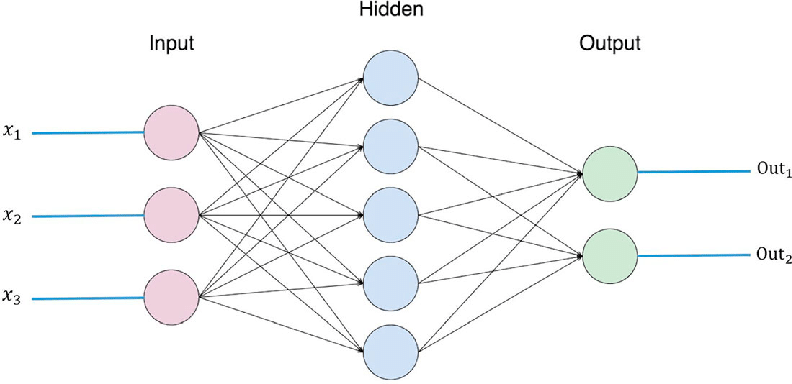
\includegraphics[scale=0.25]{theory1.png}
    \caption{A very simple one-hidden-layer Neural Network with a binary output. \newline
    In our case we have 57 attributes to input and run through with a binary output of spam/not-spam \newline
    Image Source: \cite{neuralimg1}}
    \label{fig1}
\end{figure} \newline
We can then classify our 57 attributes to either spam or not spam, and feed that back as either a correct or wrong prediction, which in turn adjusts the model (think of it as rewarding it if it gets it right) for even better results.
\subsection{Logistic Regression}
The name Logistic Regression comes from the fact that it uses a logistic function (Softmax, Sigmoid, $\tanh$ etc.) to model some binary dependent variable. In the case of spam classification, we're going to be working with a binary logistic regression model. We can then model the probability of an output given an input. This is an important thing to note, as logistic regression in itself is not a classifier, it's a regressor that can be applied to classification, for example in our binary case as:
\begin{equation}
    C(p) = \begin{cases}
                                   1 & \text{if $p(x)\geq 0.5$} \\
                                   0 & \text{otherwise}
  \end{cases}
\end{equation}
where $C$ is a class, $p$ is the probability and $x$ is an input vector with attributes. Note that $p(x)$ is (obviously) restricted to be within the confines of $p(x) \in [0,1]$. \newline
This is what enables us to use the Logistic Regression as a classification method. \newpage
Additionally, it is worth noting that Logistic Regression has a somewhat unique feature to its cost function. Normally, in a regression case, we just let this be the Mean Squared Error, however, in the case of a classification case, it is common to define the cost function as the cross entropy, given as:
\begin{equation*}
    C(\beta) = - \sum_{i=1}^n (y_i(\beta_0 + \beta_1 x_1) - \log (1+ exp(\beta_0 + \beta_1 x_1)))
\end{equation*}
The reasoning behind this is pretty clear if you think about it intuitively, given that a mean square error doesn't lend itself very well to a classification case. That is, for classification, we are not interested in what degree we missed by. We are only interested in whether we were successful or not, especially in a binary output case.\newline
The cost function is a measurement for loss. When evaluating a model, we wish for the loss (of precision) to be as small as possible. Note that since the cost function is calculated for each step, we can use it during runtime to find values with minimal loss.
\subsection{Multinominal Naïve Bayes}
Perhaps one of the most common ways of text classification, the Multinomial Naïve Bayes method is an efficient, lightweight and easy algorithm to implement. Alternatively referred to as the Multivariate Naïve Bayes, we leave our input vector (that is, attributes) as a set of frequencies for a given text string. This in turn allows us to express this as a histogram, where a multinomial \newline $\mathbf{P}$  = ($p_1, p_2, ..., p_n$) contains the probability that an event $i$ occurs.\newline The likelihood of observing a histogram $\mathbf{x}$ is given as:
\begin{equation*}
    p(\mathbf{x}|C_k) = \frac{(\sum_i x_i)!}{\prod_i x_i!} \prod_i p_{ki}^{x_i}
\end{equation*}
where $C_k$ is the total number of possible classifications, and $x_i$ is the i-th attribute in a vector containing frequencies of a given word.\newline
When then training the data set, if a classification and attribute never overlap, the frequency-based probability estimate will be zero, because the probability is directly proportional to the occurrences of a given attribute's value. \newline
Alternatively, once expressed in log-space, we instead get a linear classifier:
\begin{equation*}
    \log p(C_k | \mathbf{x}) \propto \log \left( p(C_k) \prod_{i=1}^n p_{ki}^{x_i} \right)
\end{equation*}
\begin{equation*}
    \log p(C_k | \mathbf{x}) = \log p(C_k) + \sum_{x=1}^n x_i \cdot \log p_{ki}
\end{equation*}
\begin{equation*}
    \log p(C_k | \mathbf{x}) = w_k^T \mathbf{x} + b
\end{equation*}
\newpage
\subsection{Decision Trees}
A decision tree has several layers to it. Essentially, it is built from the ground up with a root node, a set of interior nodes, and then leaf nodes off of that. The leaves themselves contain the predictions for our trained model. \newline
In layman's terms, from a top-down perspective (that is, starting at the end, from the leaf), we wish to create a model where we the leaf can predict or classify an instance. A node will specify a test of some attribute in the instance, and a branch corresponds to a possible value of an attribute. \newline
Note that an instance refers to starting first at the root node, testing the attribute specified by that node and then moving to the corresponding tree branch of the attribute value in the given input. \newline
For classification trees, we predict that each observation belongs to the most commonly occurring class in the training observations in the region to which it belongs. \newline
We will then use recursive binary splitting to grow our classification tree, but we need some sort of equivalent to a cost function. For decision trees, these are commonly called criterion, and there are three commonly used alternatives:
\newline First we have the misclassification error:
\begin{equation*}
    p_{mk} = \frac{1}{N_m} \sum_{x_i \in R_m} I(y_i \neq k) = 1 - p_{mk}
\end{equation*}
where $k$ is the number of observations in a region $R_m$ of $N_m$ total observations. The likelihood function is then represented as $I(y_i = k)$, in therms of the proportion of observations in the region $R_m$. $p$ is a probability density function.
\newline However, more commonly used are the Gini index:
\begin{equation*}
    g = \sum_{k=1}^K p_{mk}(1-p_{mk})
\end{equation*}
and the entropy:
\begin{equation*}
    s = - \sum_{k=1}^K p_{mk} \log p_{mk}
\end{equation*}
Let us also explore two common decision tree algorithms. We have first the CART algorithm.
\newline First, split the data into two subsets using some attribute $k$ and a threshold $t_k$. \newline
These values can be found by trying to minimize the cost function given as:
\begin{equation*}
    C(k, t_k) = \frac{m_l}{m}g_l + \frac{m_r}{m}g_r
\end{equation*}
where the subscript $l$ or $r$ denotes the left and right subset, respectively. The resulting two subsets will then be split, and it will keep splitting until it either reaches a user set limit or can no longer reduce the impurity of it's results. \newpage
We must also examine the ID3 algorithm.
\newline The ID3 algorithm involves very little math, and can instead be describes as list to run through:
\begin{itemize}
    \item Each instance attribute is evaluated with a statistical test to find out how well it alone classifies a training example
    \item The best found attribute from above is then chosen and used as the test root node for the tree
    \item A descendant of this root node is then created for each other possible value in the dataset for the attribute selected above
    \item Training examples are sorted into their respective descendant nodes
    \item We then repeat the process in each of these descendant nodes to find their respective best value
\end{itemize}
Resulting from this, we then get an acceptable decision tree.
\subsection{Random Forests}
For random forests, we build a number of decision trees on bootstrapped training samples, however, when building these trees, whenever a split in a tree is considered, a random sample of $m$ predictors are chosen as split candidates from our full set of predictors $p$. Note that predictor is synonymous with feature or attribute. The split is only allowed to use the one of the branched off $m$ predictors. \newline
$m$ is found in each split and is typically given as:
\begin{equation*}
    m \approx \sqrt{p}
\end{equation*}
This in turn means that at each split in a tree, our algorithm is not allowed to consider a majority of its available predictors.\newline
Imagine then that we have one very strong predictor in our data set. For such a case, the collection of bagged variable importance random forest trees, most or all of the trees will use this strong predictor in the top split. Consequently, all of the bagged trees will look quite similar to each other, in turn causing the predictions to be highly correlated. We would rather have uncorrelated quantities, as it gives us a lower variance.
\newline
The algorithm itself is pretty simple, imagine that we want to grow $B$ trees.
\begin{itemize}
    \item For b = 1 : $B$
    \begin{itemize}
        \item Draw a bootstrapped sample from our $\mathbf{X}$ training data
        \item Grow a random forest tree $T_b$ based on the selected data by repeating these three steps:
        \begin{itemize}
            \item Select $m \leq p$ variables randomly from our $p$ predictors
            \item Pick the best split point among $m$ features using a decision tree algorithm (CART/ID3)
            \item Split the node into daughter nodes
        \end{itemize}
    \end{itemize}
    \item Output the collection of trees $[T_b]_1^B$ and cast classification predictions.
\end{itemize}
\subsection{Support Vector Machines}
Support Vector Machines are another type of supervised learning model we're going to be using. Specifically, we're going to be employing the linear type of Support Vector Machines (abbreviated SVM from now). \newline
We have a data set of $x_n$ vectors corresponding to some label $y_n$. As is our case, let us now declare that $y_n$ must be integers in [0,1], meaning $y_n \in [0,1]$. 
\newline 
We wish to find the maximum-margin hyperplane that divides our $x_n$ corresponding to one value of $y_n$ (say, all $y_i = 1$) from the rest of $x_n$, such that the remainder corresponds to the other value of $y_n$. Note that a quick rundown on hyperplanes can be found in Appendix \ref{hyperp}. \newline
We have a hyperplane given as:
\begin{equation*}
    x^T w + b = 0
\end{equation*}
where $b$ is the intercept and $w$ is the elements of an orthogonal vector to the a to the linear line formed by $x^T w$. \newline
This line separates two of our given classes, and any point on it satisifes the condition:
\begin{equation*}
    x^T(w_1 - x_2) = 0
\end{equation*}
meaning that the distance $\delta$ from any point defined by some vector $x$ and a point $x_0$ must be:
\begin{equation*}
    \delta = \frac{1}{||w||}(w^T x + b)
\end{equation*}
The function to minimize is then:
\begin{equation*}
    C(w, b) = -\sum_{i\in M} y_i (x^Tw_i + b)
\end{equation*}
With the partial derivatives as:
\begin{equation*}
    \frac{\partial C}{\partial b} = -\sum_{i\in M} y_i
\end{equation*}
and
\begin{equation*}
    \frac{\partial C}{\partial w} = -\sum_{i \in M} y_i x_i 
\end{equation*}
Which can be solved by different gradient descent methods. For explanations or characteristics of these, please refer to \cite{proj2}.
\newline
There is however, another approach to solving these systems, as we can quickly run into problems implementing the results from above. 
\newline
Instead, know that any given hyperplane can be written as:
\begin{equation*}
    \Vec{w}\cdot \Vec{x} - b = 0
\end{equation*}
As discussed, we've assigned the labels 1 and 0 to mean spam and not spam. Let us instead of this example relabel not spam as -1. \newpage
This means that we get two different equations
\begin{equation*}
    \Vec{w}\cdot \Vec{x} - b \geq 1
\end{equation*}
and
\begin{equation*}
    \Vec{w}\cdot \Vec{x} - b \leq -1
\end{equation*}
which are two hyperplanes with a geometric distance of $\frac{2}{||\Vec{w}||}$, which we wish to minimize.
\newline
In turn, this means that we wish to minimize $||\Vec{w}||$ as an optimization problem for an algorithm as:
\begin{equation*}
    y_i(\Vec{w}\cdot \Vec{x}_i -b) \leq 1, \ \ \  i \in [1, n]
\end{equation*}
Note that this is a hard-margin case, that is, we assume that the data is linearly separable. If this is not the case, we will instead employ a soft-margin method, given as:
\begin{equation*}
    \max(0,1 - y_i(\Vec{w}\cdot \Vec{x}_i - b))
\end{equation*}
which means we then wish to minimize
\begin{equation*}
    \left[ \frac{1}{n} \sum_{i=1}^n \max(0, 1 - y_i(\Vec{w}\cdot \Vec{x}_i - b)) \right] + \lambda ||\Vec{w}||^2
\end{equation*}
where $\lambda$ is a parameter determining the trade-off between margin size and ensuring that $\Vec{x}_i$ is on the correct side of the boundary set by the margin.
\newline
It is also important to note that SVM is one of the more volatile methods, requiring extensive tuning of parameters in order to get desirable/good results and predictions.
\subsection{Measuring Success}
When measuring the success of a classification model, it is most common to test the accuracy of a model on the remaining test set after we've trained. 
\newline
Imagine we have a set of predictory values based on our test inputs, and the real values. We can then cast those values against each other using the following algorithm
\begin{lstlisting}[language=python]
for i in predictory:
    if i == real_data:
        corr += 1
acc = corr/len(predictory)

\end{lstlisting}
which will be an indicator of how well our model scored.
\newpage
\section{Method}
We're going to be basing our classification system off of the Spambase dataset \cite{data}, courtesy of UCI. The dataset is built up as a series of floats displaying the frequency of a given word in an e-mail, in addition to given special characters and upper case letter usage. Additionally, the data set comes pre-labeled as either spam or not spam. For a full explanation of each attribute, please refer to the UCI data set page for their documentation.\newline
We can then perform a split on our initial data set and train our models discussed above in the theory section. After this, we can (as typical of a classification problem) run our remaining test data through an accuracy function to assess the accuracy of our model. \newline
Additionally, as we wish to employ the trained method as a spam filter, we will also need to create a function that transforms a given string (e-mail) into a series of attributes akin to our original data set. We can then use our generated set of attributes to cast a binary prediction as to whether or not it is spam, and compare it against a control to compare the correct prediction rate of our different methods. \newline
As this would've been handled server side in a real life scenario, run times here are a non-issue and will therefore not be taken into consideration when weighing methods against each other. That being said, had this instead been a spam filter for an instant messaging service, we would've had to account for run times. \newline
It is also worth noting that we're going to be using Scikit and Tensorflows implementations for the most part, to read more about these please refer to appendix \ref{tensorf}
\section{Results}
First, let us examine the accuracy score of our different methods.
\newline After having sufficiently tuned all parameters of our algorithms, we calculate the accuracy over an average 10 runs to be:
\begin{table}[ht!]
    \centering
    \begin{tabular}{||c|c|c|c|c|c||}
    \hline
    \hline
         TF& LR& NB& DT& RF& SV&
    \hline
         0.94& 0.93& 0.79& 0.91& 0.95& 0.93&
    \hline
    \hline
    \end{tabular}
    \caption{A table containing all our different methods and their average values over a total of 10 runs. \newline
    Most reach and are stable at around the mid to low 90's, which in general is good. The only real outlier being NB, which can't seem to sneak past 80 accuracy score.
    \newline Which is which should be self explanatory but just in case:
    \newline TF: TensorFlow Neural Network, LR: Logistic Regression
    \newline NB: Naïve Bayes, DT: Decision Tree \newline
    RF: Random Forest, SV: Support Vector Machine}
    \label{tab1}
\end{table} \newline
We've now got a good indication as to which model can correctly assess and predict values. Let us now retool this as a makeshift email filter. \newpage
We take our trained models, and run them against a set of make-believe emails, 5 spam and 5 not spam.
\begin{table}[ht!]
    \centering
    \begin{tabular}{||c|c|c|c|c|c|c|c|c|c|c||}
    \hline
         CTRL& 1.0& 1.0& 1.0& 1.0& 1.0& 0.0& 0.0& 0.0& 0.0& 0.0  \\
    \hline
    \hline
         TF& 0.9& 1.0& 0.9& 1.0& 1.0& 0.0& 0.0& 0.0& 0.0& 0.0&
         \hline
         LR& 1.0& 1.0& 1.0& 1.0& 1.0& 0.0& 0.0& 0.0& 0.0& 0.0&
         \hline
         NB& 0.9& 1.0& 0.9& 1.0& 1.0& 0.0& 0.0& 0.0& 0.0& 0.0&
         \hline
         DT& 0.8& 0.7& 0.8& 0.6& 0.5& 0.0& 0.1& 0.0& 0.4& 0.0&
         \hline
         RF& 1.0& 1.0& 1.0& 1.0& 1.0& 0.0& 0.0& 0.0& 0.0& 0.0&
         \hline
         SV& 1.0& 1.0& 1.0& 1.0& 1.0& 0.0& 0.0& 0.0& 0.0& 0.0&
    \hline
    \end{tabular}
    \caption{A table showing all the different predictions given our "custom" spam/not spam inputs against a control. \newline
    The only methods to get a full score is Logistic Regression, Random Forest and Support Vector Machine. \newline
    Decision trees come dead last.\newline
    The "custom" string used can be found in \textsc{/data/strings.txt}}
    \label{tab2}
\end{table} \newline
Alternatively, for perhaps easier reading, we can also create a heatmap:
\begin{figure}[ht!]
    \centering
    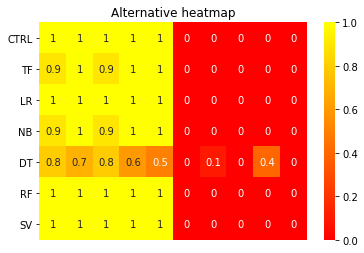
\includegraphics[scale=0.7]{heatmap.png}
    \caption{A heatmap containing the same data as seen in table [\ref{tab2}]}
    \label{fig2}
\end{figure}
\newpage
\section{Discussion}
\subsection*{Critiquing and weighing methods - what is best?}
Perhaps one of the most important qualities for our model is that it is modular, but also effective. Ideally, you'd also want it to need a minimal "starting out" dataset of system-flagged words, with additional words being added automatically by an algorithm later. Say some spam gets through and is manually flagged by a user. Given enough manually flagged data, an algorithm could then look through all manually flagged data for word correlation. If some word were to be discovered, it could be added to the database. \newline
Of course, all of our algorithms are modular, so in that sense they are all good. \newline
Let us, for simplicity's sake, rule out all but our perfect scorers in Table [\ref{tab2}], that is, Logistic Regression, Random Forest and Support Vector Machine. These are, after all, the models that were able to work effectively with the least amount of available information, that is, the input string were short and contained few words. \newline
This is where it gets a bit tricky. I specified in the method that calculation speed would be a non-factor when weighing these methods, and although that is still true, had it not been the case, Logistic Regression would've won by a landslide. From a computational standpoint, both random forest and SVM far outweigh Logistic Regression in terms of total computing time. However, looking at Table [\ref{tab1}], we can see that although all models perform admirably, Random Forest stands out as as the best performing model. \newline
It is also worth mentioning that Naïve Bayes, although it had a comparatively bad accuracy score, it performed very well with predictions. Conversely, DT had a good accuracy score, but very bad predictions. \newline
I believe therefore, that had I been able to further increase the accuracy score of the multivariate Naïve Bayes, it would've probably been on par with the greatest methods. \newline
Lastly, it is probably worth discussing the Neural Network. One would probably think that something as complex as a neural network would outperform simpler methods like Logistic Regression, but that is clearly not the case. Additionally, Neural Networks are a lot more prone to overfitting than our other methods, and requires a lot more "hands-on" continuous maintenance. Therefore I believe a Neural Network would be unsuited as a spam filter, at least when you compare it to the much simpler yet as effective other methods.
\newpage
\subsection*{Flexibility - possible expansions to the model}
There are a couple of pretty obvious way to improve on this model. Perhaps the most important one is to assign weights to given words. For example, words such as \textit{free} and \textit{money} should be given a higher priority than words like \textit{order} and \textit{make}, even though all four might appear in spam. Similarly, it would also be wise to assign weights to words that are rarely ever seen in spam. Words like \textit{conference} and \textit{table}. \newline
Additionally, it would help massively with a newer and bigger dataset. Spambase is a dataset from 1999, it is 21 years old and it shows. Even if we were to employ a spam filter as designed in this report, I doubt it would catch a lot of the spam in 2020. It would catch some, but probably not a lot. \newline
Additionally, it think it would also be beneficial to assign an extra weight to words in succession. I could probably implement this myself in my string-to-attributes converter, but it would serve little purpose when I have to create the strings myself.\newline In theory, it could look something like this:
\begin{lstlisting}[language=python]
if word in strongWords: #if word is in words with some correlation to other word, for example 'money'
    for i in range(len(strongWords)):
        if word == strongWords[i]: #get index of word
            wordIdx = i
    
    if prevWord in previous[wordIdx]: #previous holds nested lists of words correlated with strongWords[wordIdx], for example 'free'
        k += 1 #in this case, the algorithm would pick up on 'free money' which would assign extra spam weight
\end{lstlisting}
This could of course also be used both ways. A combination like 'Assignment' and 'Graded' would flag the opposite way, as not spam.
\newline This of course would take a long time as the database would likely have to be man-made, but I believe it would be an incredibly effective way of catching the most common/repetitive spam.
\subsection*{Poisoning - a fatal flaw}
A fatal flaw of this model however is that it is susceptible to poisoning. That is, poisoning the content of the email with random nonsense words that don't trigger a spam filter. \newline
This is of course because the entire model bases itself upon the frequency of a given flagged word (a bag-of-words model), so as the total number of words rises, the frequency of a flagged word decreases proportionally. 
\newline
There are two types of poisoning, based on types of statistical errors. \newline
There is a type I statistical error, where a message containing innocent words gets flagged as spam, training the filter to believe innocent words to be spam, thus causing a higher rate of false-positives.
\newline There is also a type II statistical error, where the would-be spammer includes words that typically has no place in spam, like the aforementioned "Assignment Graded", hoping to fool the filter into thinking the mail isn't spam.
\newline Additionally, there is no way for our system to catch spam where the text has been replaced with an image, unless you had an algorithm for reading text from an image, which in our case would result in machine learning upon machine learning.
\section{Conclusion}
In closing, we've shown how to create a spam filter (albeit a simple one) from the ground up various different methods. We've then weighed those methods against each other, gauging different qualities to deduce which method best fits our requirements. We've also discussed how to extend the model from a model only acting on a data set, to being able to also take any string inputs, thus preparing it for real world use, and through that found that the Random Forest method is best suited. Lastly, we've discussed and critiqued our model at length, discussing some of the most prominent weaknesses of a typical 'bag-of-words' solution.
\bibliographystyle{unsrturl}
\bibliography{citations.bib}
\newpage
\renewcommand*\appendixpagename{\Large Appendices}
\appendixpage
\addappheadtotoc
\renewcommand{\thesubsection}{\Alph{subsection}}
\subsection{Hyperplanes - A quick rundown} \label{hyperp}
What are hyperplanes? Heres a quick rundown:
\newline Hyperplanes are a subspace whose dimension is one less than that of its ambient space. This means that in an n-dimensional space, it's hyperplane would be of the $n-1$ dimension. \newline
In a technical geometric sense, it is a subspace of dimension $n-1$ in some space $V$. $V$ can be Euclidian space, affine space, a vector space or a projective space. \newline
Note that for in cases where the space $V$ is a vector space (our case), then our hyperplane is a linear subspace.
\newline Hyperplanes are a very important tool when working with Support Vector Machines \cite{hplanes}.
\subsection{Scikit and Tensorflow - Information and benefits} \label{tensorf}
\subsubsection*{Scikit and Tensorflow}
Scikit-learn is a machine learning library with a wide range of machine learning methods, ranging from classification (what we're using), regression and even clustering, using many algorithms like the ones we have discussed above, such as Support Vector machines and Random Forests. Scikit heavily used NumPy, which is of course written in C.
\subsubsection*{Tensorflow}
Tensorflow is also a library built for machine learning, but it has a particular focus on deep neural networks. Originally developed by Google for internal usage, it has since been made publicly available. It is open source, and is continuously being developed and has many practical and "high-end" uses, such as deep learning computer graphics or image captioning.
\subsubsection*{Why use these methods as opposed to our own}
The primary benefit to using these methods as opposed to creating our own is the relatively nice ease of usage. These models are very much "plug-and-play", for lack of a better term, and allow for minimal user input, outside of select parameters. This of course is very beneficial, since it allows us to spend more time on our project as opposed to bug fixes, especially in such a hectic time (exams, etc.)
\end{document}
